\section*{TP 4 - 5 : Hydrostatique}
\subsection*{Principe d'Archimède}
\begin{itemize}

	\item Soit $\overline{A}$ l'action du fluide sur le corps
		\begin{equation}
			\overline{A} = \oint _S (-p) \overline{n} \, dS 
		\end{equation}
	
	\item Equilibre du corps immergé : $\overline{A} + \overline{R} = 0$
	\item $\overline{R}$ : Résultante des forces exercées sur le corps sous l'action du fluide
	\item $\overline{A}$ : Résultante des forces de pression exercées par le fluide sur le corps
	\item \textbf{Postulat} : \textit{L'équilibre ne change pas si on remplace le corps immergé par du fluide}
		\begin{equation}
			\int _V -\rho _f g \overline{1}_z \, dV + \overline{A} = 0 \quad \Rightarrow \quad \overline{A} = \int _V \rho _f g \overline{1}_z \, dV
		\end{equation}
	\item \textbf{Attention} : il faut que tout le volume soit immergé pour appliquer Archimède
\end{itemize}

\subsection*{Principe de Pascal}

	\begin{equation}
		p + \rho g z = cst
	\end{equation}
	\noindent Si en un point du fluide incompressible en équilibre isotherme, la pression est accrue de $\Delta p$, tous les points subissent cet accroissement

\subsection*{Répartition des pressions sur un obstacle}
\begin{itemize}
\item La pression est toujours orienté selon la normale à la surface
\item On choisit une pression de référence : $p_{ref} = 0$ ou $p_{ref} = p_{atm} = 101325 \, Pa$
\item On trouve l'évolution de la pression grâce au principe de Pascal
\end{itemize}
\ \\
\begin{minipage}{0.55 \textwidth}
\begin{flushleft}
	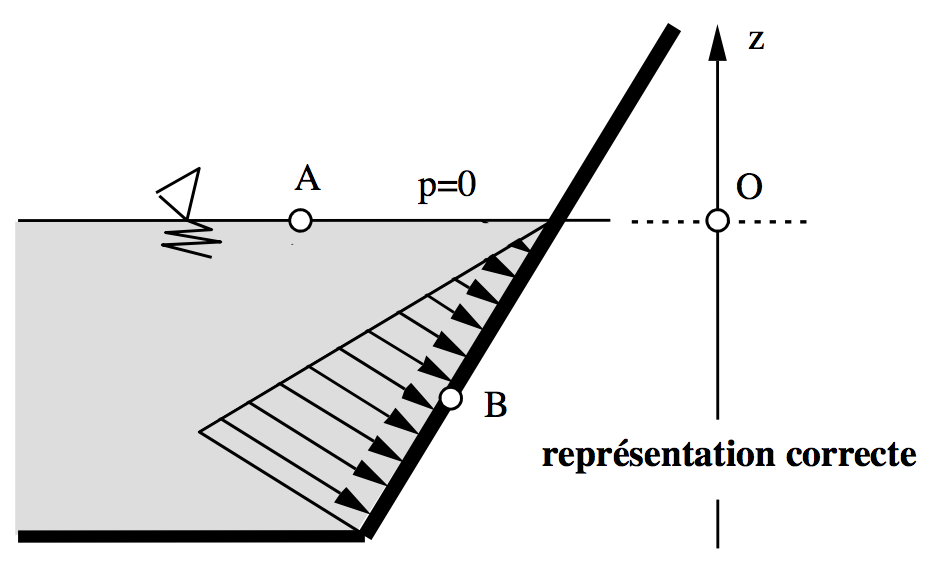
\includegraphics[scale=0.5]{tp4-1}
\end{flushleft}
\end{minipage}
\begin{minipage}{0.5 \textwidth}
\begin{flushleft}
	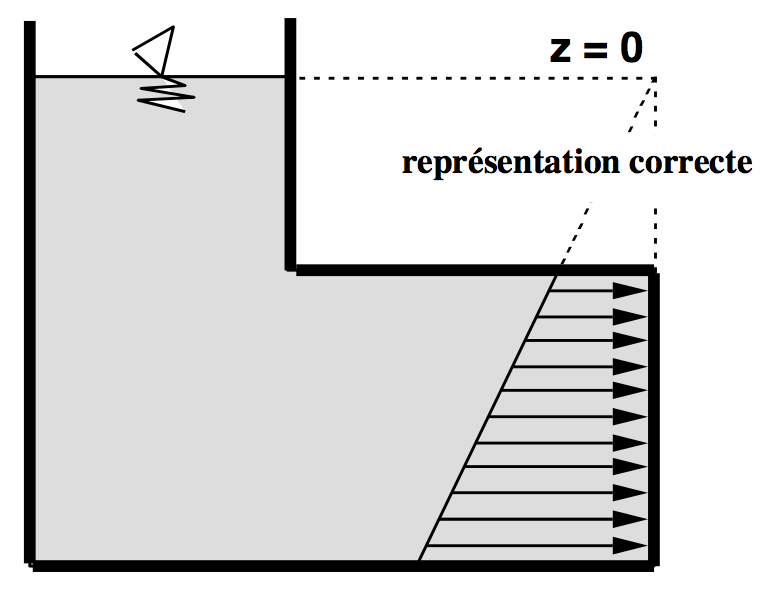
\includegraphics[scale=0.5]{tp4-2}
\end{flushleft}
\end{minipage}